% !TEX root = ../main.tex
\chapter{Koopman Spectral Analysis}\label{ch:koopman}
\begin{paracol}{2}

\begin{sources}
\begin{tabularx}{\linewidth}{@{}V l L@{}}
\toprule
\textbf{Video} & \textbf{Length} & \textbf{Content}\\
\midrule
\seg{6}{1}{V6.1 Koopman Spectral Analysis (Overview)} & 27:49 & Open problems; Koopman 1931 and the ergodic theorem; the operator on observables; eigenfunctions and invariant subspaces; the slow-manifold example; $\dot x=x^2$ and $e^{-1/x}$; the eigenfunction PDE; DMD as an approximation.\\
\seg{6}{2}{V6.2 Koopman Spectral Analysis (Representations)} & 16:01 & Extended DMD; overfitting and VAC; sparse identification of eigenfunctions; deep Koopman autoencoders; error versus complexity; cross-validation.\\
\seg{6}{3}{V6.3 Koopman Spectral Analysis (Control)} & 15:26 & LQR in Koopman coordinates; control of eigenfunctions (energy); state-dependent Riccati; well hopping and space missions; double gyre; other Koopman-control methods.\\
\seg{6}{4}{V6.4 Koopman Spectral Analysis (Continuous Spectrum)} & 12:43 & Chaos and HAVOK; the pendulum and its continuous spectrum; autoencoders with an auxiliary network; action-angle coordinates.\\
\seg{6}{5}{V6.5 Koopman Spectral Analysis (Multiscale systems)} & 5:08 & Delay coordinates for multiscale systems (coupled van der Pol); multiresolution DMD; summary.\\
\bottomrule
\end{tabularx}

\smallskip
\textbf{Transcripts} \file{materials/transcripts/C06-V0*.txt}.
\textbf{Book} Sec.~7.4 (Koopman operator theory), Sec.~7.5 (data-driven Koopman analysis).
\textbf{Code} \file{code/ch06_koopman.py}.
\end{sources}

\section*{Motivation}
The first primary challenge of \cref{ch:overview} was nonlinearity. Koopman theory attacks it with a
change of point of view: instead of the state, follow the \emph{measurements} of the state. On the space of
all possible measurements the dynamics acts \emph{linearly}, through an infinite-dimensional operator
\ts{6}{1}{5:29}. The price is the dimension; the game of modern data-driven Koopman theory is to find a few
special measurements, the eigenfunctions, in which a nonlinear system looks linear, and then use textbook
linear tools for prediction, estimation and control. A physicist has met this before: the Heisenberg
picture, where observables evolve and states stay put, and action-angle variables, where an integrable
system becomes uniform rotation.

The open problems that frame the series \ts{6}{1}{2:04}: unknown equations (no equation for the brain, the
climate or an epidemic) \ts{6}{1}{2:25}; nonlinearity, where even a quadratic term confounds understanding
\ts{6}{1}{3:05}; control (Brunton is a control theorist) \ts{6}{1}{3:26}; chaos, transients and intermittency
\ts{6}{1}{3:46}; multiscale physics \ts{6}{1}{4:07}; and, not treated here, noise and uncertainty \ts{6}{1}{4:48}.

% ------------------------------------------------------------------
\section{The Koopman operator}\label{sec:ko-operator}

\begin{history}[Koopman, von Neumann, Birkhoff]
Bernard O.~Koopman, \emph{Hamiltonian systems and transformation in Hilbert space}, PNAS 17 (1931) 315--318,
observed that a Hamiltonian flow induces a \emph{unitary} operator on $L^2$ functions of phase space
(Liouville's theorem preserves the measure). Within months John von Neumann used it to prove the mean
ergodic theorem, and George D.~Birkhoff the pointwise one (PNAS, 1931--32), a priority race that left
bruises; Koopman and von Neumann also wrote a joint paper (1932) on systems with continuous spectrum. The
operator view then slept for decades, while Poincar\'e's geometric view dominated, until Igor Mezi\'c and
co-workers revived it (1999--2005) \ts{6}{1}{5:50}\ts{6}{1}{8:14}\ts{6}{1}{8:56}.\par
\textit{References:} C.~C.~Moore, \emph{Ergodic theorem, ergodic theory, and statistical mechanics},
PNAS 112 (2015) 1907--1911 (the perspective recommended in the video); I.~Mezi\'c, Nonlinear Dyn.\ 41 (2005).
\end{history}

Koopman considered the Hilbert space of all possible measurements of the system: not only $x$, but $x^2$,
$\cos x$, $\arctan x$, \dots\ In that infinite-dimensional space the nonlinear dynamics is a linear operator
that advances measurements in time \ts{6}{1}{6:32}\ts{6}{1}{6:52}\ts{6}{1}{7:13}. ``Measurement'' is a fancy
word for data, which is why the 1931 idea fits the data-science era \ts{6}{1}{7:33}\ts{6}{1}{7:54}.

\begin{definition}[New concepts: observable, Koopman operator]\label{def:ko-op}
An \textbf{observable} is a function $g:M\to\C$ of the state (in a suitable function space, e.g.\
$L^2$). For the discrete-time system $\vb x_{k+1}=\vb F(\vb x_k)$ (or the flow map $\vb F_t$) the
\textbf{Koopman operator} acts on observables by composition:
\begin{equation}\label{eq:ko-def}
  \K g=g\circ\vb F,\qquad\text{i.e.}\qquad (\K g)(\vb x_k)=g(\vb x_{k+1});
\end{equation}
in continuous time $\K^tg=g\circ\vb F_t$, with generator $\mathcal Lg=\lim_{t\to0}(\K^tg-g)/t=\nabla g\cdot\vb f$.
$\K$ is \emph{linear}, $\K(ag_1+bg_2)=a\K g_1+b\K g_2$, however nonlinear $\vb F$ is
\ts{6}{1}{10:59}\ts{6}{1}{11:19}. It is named after B.~O.~Koopman; its adjoint, acting on densities, is the
Perron--Frobenius (transfer) operator.
\end{definition}

Geometric view: trajectories in state space, fixed points, manifolds, attractors. Operator view: how
measurements evolve \ts{6}{1}{10:18}\ts{6}{1}{10:39}. The trade: a finite-dimensional nonlinear problem for an
infinite-dimensional linear one \ts{6}{1}{7:13}. Finding finite-dimensional approximations (matrices) of
$\K$ has been the subject of intense research for a decade \ts{6}{1}{11:40}\ts{6}{1}{12:00}.

\begin{definition}[New concepts: Koopman eigenfunction, invariant subspace]\label{def:ko-eig}
A \textbf{Koopman eigenfunction} is an observable $\varphi$ with $\K\varphi=\mu\varphi$, i.e.\
$\varphi(\vb x_{k+1})=\mu\varphi(\vb x_k)$: measured in $\varphi$, the system evolves exactly linearly,
as a pure exponential or oscillation \ts{6}{1}{12:20}. In continuous time
$\frac{\mathrm d}{\mathrm dt}\varphi(\vb x)=\lambda\varphi(\vb x)$, $\mu=e^{\lambda\Delta t}$. A subspace of
observables spanned by $\{g_1,\dots,g_p\}$ is \textbf{Koopman invariant} if $\K g_j$ stays in the span for
every $j$; eigenfunctions span such subspaces, and restricted to one, $\K$ is a $p\times p$ matrix
\ts{6}{1}{12:42}\ts{6}{1}{13:02}.
\end{definition}

\begin{proposition}[Eigenfunction PDE]\label{prop:ko-pde}
A smooth eigenfunction of the flow of $\dot{\vb x}=\vb f(\vb x)$ satisfies the linear first-order PDE
\begin{equation}\label{eq:ko-pde}
  \nabla\varphi(\vb x)\cdot\vb f(\vb x)=\lambda\,\varphi(\vb x).
\end{equation}
Products of eigenfunctions are eigenfunctions: $\varphi_1\varphi_2$ has eigenvalue $\lambda_1+\lambda_2$.
\end{proposition}
\begin{proof}
Chain rule: $\frac{\mathrm d}{\mathrm dt}\varphi(\vb x(t))=\nabla\varphi\cdot\dot{\vb x}=\nabla\varphi\cdot\vb f$,
which must equal $\lambda\varphi$ along every trajectory, hence everywhere \ts{6}{1}{18:55}\ts{6}{1}{19:16}\ts{6}{1}{19:37}.
For the product, $\nabla(\varphi_1\varphi_2)\cdot\vb f=\varphi_2\lambda_1\varphi_1+\varphi_1\lambda_2\varphi_2$.
\end{proof}

\begin{example}[Linear systems]
For $\dot{\vb x}=A\vb x$ with left eigenvectors $\vb w_j^*A=\lambda_j\vb w_j^*$, the linear observables
$\varphi_j(\vb x)=\vb w_j^*\vb x$ are eigenfunctions: $\dot\varphi_j=\vb w_j^*A\vb x=\lambda_j\varphi_j$.
These are the coordinates $\vb z=T^{-1}\vb x$ of \cref{prop:ov-linear}. Koopman eigenfunctions
generalize eigenvector coordinates to nonlinear systems.
\end{example}

% ------------------------------------------------------------------
\section{Two examples: closure and non-closure}\label{sec:ko-examples}

\begin{casestudy}[A slow manifold made linear]
The system of \cref{ex:fu-saddle} (the book's Sec.~7.4 example) \ts{6}{1}{13:02}\ts{6}{1}{13:23}:
\begin{equation}\label{eq:ko-slow}
  \dot x_1=\mu x_1,\qquad \dot x_2=\lambda(x_2-x_1^2).
\end{equation}
If $\lambda$ is much more negative than $\mu$, $x_2$ quickly relaxes to $x_1^2$: trajectories stick to the
slow manifold $x_2=x_1^2$ and slide to the origin \ts{6}{1}{13:23}\ts{6}{1}{13:43}. Add the nonlinear
measurement $y_3=x_1^2$ to $y_1=x_1$, $y_2=x_2$ \ts{6}{1}{13:43}\ts{6}{1}{14:04}:
\[
  \dot y_1=\mu y_1,\quad \dot y_2=\lambda y_2-\lambda y_3,\quad \dot y_3=2x_1\dot x_1=2\mu y_3,
  \qquad
  \frac{\mathrm d}{\mathrm dt}\vb y=\begin{bmatrix}\mu&0&0\\0&\lambda&-\lambda\\0&0&2\mu\end{bmatrix}\vb y .
\]
An honest $3\times3$ linear system: it predicts the nonlinear dynamics as far ahead as wanted with a matrix
exponential, and projected on $(y_1,y_2)$ reproduces the slow-manifold behaviour
\ts{6}{1}{14:25}\ts{6}{1}{14:45}\ts{6}{1}{15:06}\ts{6}{1}{15:27}. Eigenfunctions:
$\varphi_\mu=x_1$, $\varphi_{2\mu}=x_1^2$, and $\varphi_\lambda=x_2-bx_1^2$ with $b=\lambda/(\lambda-2\mu)$;
the level set $\varphi_\lambda=0$ is the unstable/slow manifold found in \cref{ex:fu-saddle}.
\end{casestudy}

\paragraph{When it does not close: $\dot x=x^2$.} Even simpler, and nasty: finite-time blow-up (``you can't
say this in an airport'') \ts{6}{1}{15:49}\ts{6}{1}{16:09}. With $y_1=x$, $y_2=x^2$: $\dot y_1=y_2$, but
$\dot y_2=2x\dot x=2x^3$, outside the span; adding $x^3$ produces $x^4$, and so on forever
\ts{6}{1}{16:30}\ts{6}{1}{16:50}. Truncations converge slowly to the true solution \ts{6}{1}{17:12}. Lesson: an
arbitrary Taylor or Fourier basis is usually a bad basis; the right representation is in terms of
eigenfunctions \ts{6}{1}{17:32}. And there is one (Clancy Rowley wrote it down while waiting for a bus)
\ts{6}{1}{17:53}:
\[
  \varphi(x)=e^{-1/x},\qquad \dot\varphi=\frac{\dot x}{x^2}e^{-1/x}=\varphi ,
\]
an eigenfunction with $\lambda=1$, not representable by a finite Taylor series (it is the textbook
non-analytic smooth function) \ts{6}{1}{18:14}. Solving \eqref{eq:ko-pde} with a Laurent series ansatz,
powers $x^k$ and $x^{-k}$, produces exactly this function \ts{6}{1}{19:59}\ts{6}{1}{20:20}\ts{6}{1}{20:41}.

\begin{intuition}[Eigenfunctions are clocks]
$\varphi=e^{-1/x}$ is $e^{t}$ up to a constant: it measures elapsed time. Indeed $-1/x$ grows by exactly 1 per
unit time ($\frac{\mathrm d}{\mathrm dt}(-1/x)=1$), the ``uniform motion'' coordinate of \cref{ch:overview}.
Every eigenfunction with $\operatorname{Re}\lambda\ne0$ is $e^{\lambda\tau(\vb x)}$ for some ``time function''
$\tau$ with $\dot\tau=1$; with $\lambda=i\omega$ it is a phase. Finding eigenfunctions means finding
coordinates in which time flows uniformly.
\end{intuition}

\codefile{Koopman examples}{../code/ch06_koopman.py}

% ------------------------------------------------------------------
\section{Data-driven approximations}\label{sec:ko-data}

\paragraph{DMD.} The workhorse: the best-fit linear operator $A$ between snapshot matrices is a
finite-dimensional approximation of $\K$ restricted to \emph{linear} observables of the state; the
connection was made by Rowley, Mezi\'c et al.\ (2009) on a jet in cross flow
\ts{6}{1}{21:23}\ts{6}{1}{21:43}\ts{6}{1}{22:04}\ts{6}{1}{25:32}. It works remarkably well for periodic or
quasi-periodic data, less well for transients and intermittency \ts{6}{1}{23:27}\ts{6}{1}{23:48}. Further
connections in fluids: Bagheri's Koopman analysis of the cylinder wake, and the link with resolvent analysis
(Sharma, Mezi\'c, McKeon) \ts{6}{1}{25:52}\ts{6}{1}{26:13}\ts{6}{1}{26:33}.

\paragraph{Extended DMD.} Williams, Kevrekidis and Rowley (2015): a linear model cannot have multiple fixed
points or genuinely nonlinear transients \ts{6}{2}{2:26}, so augment the state with nonlinear observables
(monomials, $\cos x$, radial basis functions, Bessel functions) and fit the best linear operator on the
augmented state \ts{6}{2}{2:47}\ts{6}{2}{3:07}. On the Duffing oscillator it finds eigenfunctions where DMD
fails \ts{6}{2}{3:28}\ts{6}{2}{3:48}.
\begin{definition}[New concepts: extended DMD]
With a dictionary $\boldsymbol\psi(\vb x)=(\psi_1(\vb x),\dots,\psi_p(\vb x))^{\mathsf T}$ and snapshot pairs
$(\vb x_k,\vb x_k')$, form $\Psi=[\boldsymbol\psi(\vb x_1)\cdots]$, $\Psi'=[\boldsymbol\psi(\vb x_1')\cdots]$
and $K=\Psi'\Psi^\dagger$, the least-squares approximation of $\K$ on the span of the dictionary. Eigenvectors
$\vb v$ of $K^{\mathsf T}$ give approximate eigenfunctions $\varphi(\vb x)=\vb v^{\mathsf T}\boldsymbol\psi(\vb x)$.
\end{definition}

In the script, EDMD with the 10 monomials of degree $\le3$ on \eqref{eq:ko-slow} ($\mu=-0.05$, $\lambda=-1$)
returns the exact eigenvalues $0,\mu,2\mu,3\mu,\lambda,\lambda+\mu$ ($0,-0.05,-0.1,-0.15,-1,-1.05$) and four
\emph{spurious} ones ($-1.48$, a complex pair, $-1.89$, $-3.05$): eigenfunctions such as $\varphi_\lambda^2$ need $x_1^4$,
which is not in the dictionary, and the regression returns its best but wrong guess.

\paragraph{Overfitting.} A huge dictionary means a huge matrix with many free parameters: massive
overfitting unless one cross-validates \ts{6}{2}{4:09}\ts{6}{2}{4:29}. The variational approach to conformation
dynamics (VAC) of Frank No\'e and co-workers (2013) builds cross-validation in, through a ``VAC score''
\ts{6}{2}{4:51}\ts{6}{2}{15:09}.

\paragraph{Sparse eigenfunctions.} Eurika Kaiser's alternative: skip the big matrix, whose eigenvectors are
often spurious, and look for eigenfunctions directly, sparse in a library $\Theta$, $\varphi(\vb x)=\Theta(\vb x)\vb c$
\ts{6}{2}{5:11}\ts{6}{2}{5:32}\ts{6}{2}{5:53}\ts{6}{2}{6:13}. Evaluating \eqref{eq:ko-pde} on data gives
$\big(\Gamma(\vb x,\dot{\vb x})-\lambda\Theta(\vb x)\big)\vb c=0$, with $\Gamma=\nabla\Theta\cdot\dot{\vb x}$: a sparse
vector in a null space \ts{6}{2}{6:54}\ts{6}{2}{7:15}. One must know $\lambda$ roughly, but lightly damped
eigenfunctions ($\operatorname{Re}\lambda\approx0$) persist in the data and are the easiest to find, and they are
also the ones that matter for prediction and control \ts{6}{2}{7:35}\ts{6}{2}{7:56}. Conserved quantities are
eigenfunctions with $\lambda=0$: from Duffing data the method discovers the Hamiltonian \ts{6}{2}{8:16}\ts{6}{2}{9:18}.
In discrete time the same idea gives back VAC and EDMD, or sparse versions of them \ts{6}{2}{8:36}.

\paragraph{Deep Koopman.} Neural networks represent complicated functions well when data are plentiful
\ts{6}{2}{11:02}. Many groups (Lusch, Kutz and Brunton among them) use an autoencoder: an encoder $\varphi$ to a few
latent variables, a decoder $\varphi^{-1}$ back to the state, and a \emph{linear} time-stepper $K$ in the
latent space \ts{6}{2}{10:00}\ts{6}{2}{10:20}\ts{6}{2}{10:42}. The field moves fast \ts{6}{2}{11:23}.

\begin{intuition}[Error versus complexity]
Plot model error against complexity \ts{6}{2}{11:43}\ts{6}{2}{12:04}. Exact Koopman theory is the ``unicorn''
on the far right: perfect linearization, infinite complexity. DMD is on the left: simple, good for periodic
data, poor for transients and chaos \ts{6}{2}{12:25}\ts{6}{2}{12:45}. The hope is a curved Pareto front with a
sweet spot of low complexity and good error \ts{6}{2}{13:05}\ts{6}{2}{13:25}. But on \emph{training} data any
EDMD or network can reach zero error; only \emph{cross-validated} error on held-out trajectories reveals the
front. ``You will get garbage models if you don't cross validate'' \ts{6}{2}{13:46}\ts{6}{2}{14:06}\ts{6}{2}{14:27}.
Sparse methods are parsimonious by construction \ts{6}{2}{14:48}.
\end{intuition}

% ------------------------------------------------------------------
\section{Koopman and control}\label{sec:ko-control}

The promise: in Koopman coordinates, textbook linear control (LQR, Kalman filters, ``one-line commands in
Matlab'') works for strongly nonlinear systems; finding the coordinates is an up-front cost, everything
downstream is easy \ts{6}{3}{0:42}\ts{6}{3}{1:03}. For \eqref{eq:ko-slow} with a control $u$ on $x_2$, the lifted
system is $\dot{\vb y}=K\vb y+Bu$; LQR on it returns three gains, and the gain on $y_3=x_1^2$ is a
\emph{nonlinear} feedback in the original variables. It is about three times cheaper (in the LQR cost) than
LQR on the linearization at the origin, because it exploits the slow manifold instead of fighting it
\ts{6}{3}{2:06}\ts{6}{3}{2:26}\ts{6}{3}{3:07}\ts{6}{3}{3:48}\ts{6}{3}{4:09}\ts{6}{3}{4:29}. Chapter~7 works this example
out. The pipeline: data $\to$ model (DMD, SINDy) $\to$ Koopman coordinates $\to$ linear optimal control
\ts{6}{3}{4:49}\ts{6}{3}{5:51}.

\paragraph{Control in eigenfunction coordinates.} With $\dot{\vb x}=\vb f(\vb x)+B\vb u$ and eigenfunctions
$\varphi$ of the \emph{unforced} system \ts{6}{3}{6:12}\ts{6}{3}{6:32}:
\begin{equation}\label{eq:ko-control}
  \dot\varphi=\nabla\varphi\cdot(\vb f+B\vb u)=\lambda\varphi+\nabla\varphi(\vb x)\cdot B\vb u .
\end{equation}
The dynamics stays linear in $\varphi$; only the actuation becomes state dependent: the actuator is more or
less effective depending on where the state is \ts{6}{3}{6:53}\ts{6}{3}{7:13}\ts{6}{3}{7:34}. One then steers the
eigenfunctions themselves \ts{6}{3}{8:16}. For a conservative system the energy $H$ is an eigenfunction
($\lambda=0$): to swing up a pendulum, drive $H$ to the energy of the upright position instead of driving the
state to $(\pi,0)$ \ts{6}{3}{8:37}\ts{6}{3}{8:58}. The control is solved with a state-dependent Riccati equation
(SDRE) \ts{6}{3}{9:18}\ts{6}{3}{9:39}.

\begin{application}[Well hopping and the Jupiter icy moons]
Eurika Kaiser found, purely from data, the energy eigenfunctions of a quartic well, the Duffing oscillator and
the pendulum, and designed controllers that move the energy up or down \ts{6}{3}{10:00}\ts{6}{3}{10:21}; with
multiple wells, two controllers in sequence push the system over the barrier and settle it in the next well
\ts{6}{3}{10:42}\ts{6}{3}{11:02}. This is the problem of energy-efficient space missions: each planet and moon is a
potential well inside the Sun's; touring the moons of Jupiter means hopping between wells (the \emph{Jupiter
Icy Moons Orbiter} studies, on which Brunton's undergraduate advisor Jerry Marsden worked)
\ts{6}{3}{11:22}\ts{6}{3}{11:43}\ts{6}{3}{12:04}. A higher-dimensional example: a double-gyre ocean model, where
the method stabilizes coordinated swarms of drifters \ts{6}{3}{12:25}\ts{6}{3}{12:46}.
\end{application}

Other Koopman-control work: Koopman Kalman filters (A.~Surana), model predictive control on EDMD models (M.~Korda,
I.~Mezi\'c), also for power-grid stabilization, and switching between Koopman models built for fixed
control values (S.~Peitz and co-workers) \ts{6}{3}{13:49}\ts{6}{3}{14:11}\ts{6}{3}{14:32}.

% ------------------------------------------------------------------
\section{Continuous spectrum and multiscale systems}\label{sec:ko-continuous}

\paragraph{Chaos.} The Fourier transform of a long Lorenz signal has a continuous power spectrum: no finite
set of eigenvalues represents it \ts{6}{4}{0:43}\ts{6}{4}{1:04}. The HAVOK method (Chapter~8) found that
delay coordinates make even chaotic dynamics almost linear, with an intermittent forcing that signals the lobe
switches \ts{6}{4}{1:24}\ts{6}{4}{2:27}\ts{6}{4}{2:48}\ts{6}{4}{3:09}\ts{6}{4}{3:31}.

\paragraph{The pendulum.} It frustrated Brunton that Koopman theory was applied to turbulence and the brain
while nobody could write down the Koopman eigenfunctions of a pendulum \ts{6}{4}{4:12}\ts{6}{4}{4:32}. The
reason is a \emph{continuous spectrum}: a small kick gives pure oscillations at the natural frequency, but the
period grows with the energy and tends to infinity at the separatrix, so the frequency deforms continuously
from $\omega_0$ to 0, and there are no isolated eigenvalues \ts{6}{4}{5:13}\ts{6}{4}{5:34}\ts{6}{4}{5:54}.

\begin{proposition}[Frequency of the pendulum]\label{prop:ko-pendulum}
For $\ddot\theta=-\sin\theta$ ($g/L=1$) at energy $E=\frac12\dot\theta^2-\cos\theta\in(-1,1)$, the libration
frequency is
\[
  \omega(E)=\frac{\pi}{2K(k)},\qquad k^2=\frac{1+E}{2},
\]
with $K$ the complete elliptic integral of the first kind; $\omega\to1$ as $E\to-1$ and $\omega\to0$ as $E\to1$.
\end{proposition}
\begin{proof}
The period is $T=4\int_0^{\theta_m}\mathrm d\theta/\sqrt{2(E+\cos\theta)}$ with $\cos\theta_m=-E$. Using
$E+\cos\theta=2(k^2-\sin^2\frac\theta2)$ and the substitution $\sin\frac\theta2=k\sin s$ gives $T=4K(k)$, so
$\omega=2\pi/T=\pi/(2K)$. $K(0)=\pi/2$, and $K(k)\sim\ln(4/\sqrt{1-k^2})\to\infty$ as $k\to1$.
\end{proof}

\begin{nfigure}
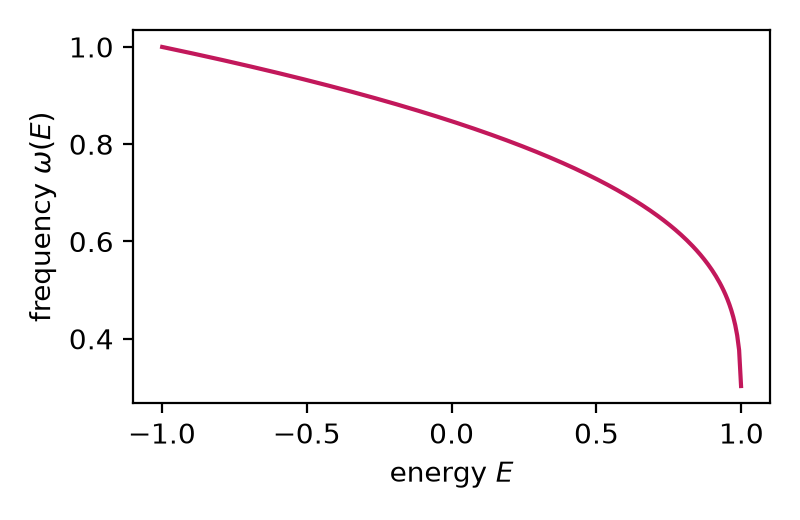
\includegraphics[width=0.42\linewidth]{figures/ch06-pendulum-omega.png}
\caption{Output of \file{ch06_koopman.py}: the pendulum frequency $\omega(E)$ of
\cref{prop:ko-pendulum}, from $1$ at the bottom to $0$ at the separatrix. Each energy level carries its own
pair of eigenvalues $\pm i\omega(E)$: a continuum.}\label{fig:ko-omega}
\end{nfigure}

\paragraph{Parametrized autoencoders.} A Koopman autoencoder whose middle matrix has fixed eigenvalues $\pm i\omega$
cannot represent this; it would need all harmonics $\pm i\omega,\pm2i\omega,\dots$ and a big latent layer
\ts{6}{4}{6:35}\ts{6}{4}{6:55}\ts{6}{4}{7:16}\ts{6}{4}{7:37}\ts{6}{4}{7:57}. Bethany Lusch added an auxiliary network that
learns $\omega$ as a function of the state (in effect of the energy), keeping a $2\times2$ Jordan-block structure
with eigenvalues $\pm i\omega$ \ts{6}{4}{8:17}\ts{6}{4}{8:38}\ts{6}{4}{8:59}. The learned eigenfunctions map the
pendulum to perfect sines and cosines whose frequency depends on the amplitude \ts{6}{4}{9:20}\ts{6}{4}{9:41};
in magnitude and phase they are the action-angle coordinates of classical mechanics, as Mezi\'c pointed out
\ts{6}{4}{10:01}\ts{6}{4}{10:21}. It scales to the cylinder wake \ts{6}{4}{10:42}\ts{6}{4}{11:03}.

\begin{intuition}[Action-angle variables are Koopman eigenfunctions]
For an integrable system with actions $I$ and angles $\vartheta$, $\dot I=0$ and $\dot\vartheta=\omega(I)$. So any
function of $I$ is an eigenfunction with $\lambda=0$, and $h(I)e^{i\vartheta}$ satisfies
$\frac{\mathrm d}{\mathrm dt}=i\omega(I)\,h(I)e^{i\vartheta}$: an eigenfunction only on each torus, with an
eigenvalue that depends on the torus. That is the continuous spectrum, and it is why the auxiliary network
must output $\omega(I)$.
\end{intuition}

Continuous spectra are ubiquitous: most systems of interest have eigenvalues that deform continuously with
energy or control inputs \ts{6}{4}{11:24}\ts{6}{4}{11:44}. The two leading tools are delay coordinates and deep
(parametrized) autoencoders \ts{6}{4}{12:04}\ts{6}{4}{12:25}.

\paragraph{Multiscale systems.} Kathleen Champion: DMD on delay coordinates gives nearly perfect closed linear
models of quasi-periodic van der Pol, Lorenz and R\"ossler oscillators, improving with the rank and the delay
\ts{6}{5}{1:04}\ts{6}{5}{1:25}\ts{6}{5}{1:46}; with a slow and a fast van der Pol oscillator coupled, it separates the
time scales from the single measurement $x_1+x_2$ \ts{6}{5}{2:06}\ts{6}{5}{2:27}. Kutz's multiresolution DMD pulls
out intermittent phenomena such as El Ni\~no from sea-surface temperature \ts{6}{5}{2:27}\ts{6}{5}{2:48}.
Summary: regression methods (DMD, EDMD, sparse eigenfunctions, networks) find coordinates in which a nonlinear
system is linear; the coordinates are a one-time cost that pays off downstream in control; open questions are
scaling, where it works, and whether the up-front cost is worth it \ts{6}{5}{3:08}\ts{6}{5}{3:29}\ts{6}{5}{4:10}.

\begin{keyformulas}
\begin{itemize}
  \item $\K g=g\circ\vb F$ (linear); generator $\mathcal Lg=\nabla g\cdot\vb f$.
  \item Eigenfunctions $\K\varphi=\mu\varphi$, $\nabla\varphi\cdot\vb f=\lambda\varphi$; products add eigenvalues.
  \item Slow manifold: $(x_1,x_2,x_1^2)$ closes, $K=\begin{psmallmatrix}\mu&0&0\\0&\lambda&-\lambda\\0&0&2\mu\end{psmallmatrix}$;
        $\dot x=x^2$: $\varphi=e^{-1/x}$, $\lambda=1$.
  \item EDMD $K=\Psi'\Psi^\dagger$; cross-validate. Control: $\dot\varphi=\lambda\varphi+\nabla\varphi\cdot B\vb u$.
  \item Pendulum: $\omega(E)=\pi/2K(k)$, continuous spectrum; action-angle variables.
\end{itemize}
\end{keyformulas}

\section*{Exercises}

\begin{exercise}[Koopman operator of a map]
For the linear map $x_{k+1}=ax_k$ find all polynomial eigenfunctions of $\K$ and their eigenvalues. For the
doubling map $x_{k+1}=2x_k\bmod1$ on $[0,1)$, show that $e^{2\pi i\,2^nx}$ is mapped by $\K$ to $e^{2\pi i2^{n+1}x}$:
$\K$ is a shift on Fourier modes, with no eigenfunction other than constants in $L^2$.
\end{exercise}

\begin{exercise}[Laurent series]
Insert $\varphi(x)=\sum_{k=-\infty}^{\infty}c_kx^k$ into \eqref{eq:ko-pde} for $f(x)=x^2$, derive the recursion for
the coefficients, and show that the solution with $\lambda=1$ is $e^{-1/x}$. What are the eigenfunctions for
other $\lambda$?
\end{exercise}

\begin{exercise}[Eigenfunctions of the slow-manifold system]
Verify that $x_2-\frac{\lambda}{\lambda-2\mu}x_1^2$ is an eigenfunction of \eqref{eq:ko-slow}. Find the eigenvectors
of $K$ and relate them to the eigenfunctions. Then run the EDMD part of \file{ch06_koopman.py} with monomials up
to degree 4 and 5: which spurious eigenvalues disappear?
\end{exercise}

\begin{exercise}[Energy as an eigenfunction]
Show that for any Hamiltonian system $H$ is a Koopman eigenfunction with $\lambda=0$, and so is any function of
$H$. Write \eqref{eq:ko-control} for the pendulum with a torque $u$ and derive the energy-pumping law
$u=-k\,\dot\theta\,(H-H^*)$ from $\frac{\mathrm d}{\mathrm dt}\frac12(H-H^*)^2\le0$.
\end{exercise}

\begin{exercise}[Spectrum of a signal]
Compute the power spectrum of $x(t)$ for Lorenz (from \file{ch03_lorenz.py}) and for the pendulum at two energies.
Compare the broadband Lorenz spectrum with the lines of the pendulum. What happens to the pendulum spectrum if
the record is an ensemble over many energies?
\end{exercise}

\end{paracol}
